\section{Experiments}

\subsection{Single-split model selection is optimistic}
\label{sec:protocol-study}
A common way to tune classifiers on a small dataset is to standardize the features of all patients, draw one stratified 5-fold split, score every configuration of a grid on it, and report the best score. We applied this protocol to standard classifiers on the 21 volumetric features (true LV), with grids of 12 to 135 configurations, and compared it with nested cross-validation on the same grids (Table~\ref{tab:protocol-study}).

% Generated by regenerate_figures.py from final/results/protocol_study
\begin{table}[!htb]
\centering
\small
\setlength{\tabcolsep}{4pt}
\begin{adjustbox}{max width=\linewidth}
\begin{tabular}{lrrrrr}
\toprule
& \multicolumn{4}{c}{Single split (scaler fitted on all patients)} & \\
\cmidrule(lr){2-5}
Model & Configs & Tied best & Median & Best & Nested CV\\
\midrule
Random forest & 30 & 12 & 0.930 & 0.940 & 0.930 $\pm$ 0.012\\
XGBoost & 135 & 97 & 0.910 & 0.910 & 0.910 $\pm$ 0.007\\
SVM (linear or RBF) & 12 & 2 & 0.925 & 0.950 & 0.936 $\pm$ 0.009\\
$k$-NN & 16 & 3 & 0.880 & 0.930 & 0.904 $\pm$ 0.021\\
MLP ensemble & -- & -- & -- & 0.936 & 0.926 $\pm$ 0.011\\
MLP + RF & 11 & -- & -- & 0.938 & 0.926 $\pm$ 0.005\\
MLP + linear SVM & 11 & -- & -- & 0.938 & 0.932 $\pm$ 0.008\\
\bottomrule
\end{tabular}
\end{adjustbox}
\caption{Model selection on a single split vs nested cross-validation (21 volumetric features, true LV).
\emph{Single split}: every configuration of the grid scored on one stratified 5-fold split; \emph{Best}: the best
of them, \emph{Tied best}: number of configurations reaching it, \emph{Median}: median over the grid. For the
MLP ensemble (no grid), mean over 5 seeds; for the soft votes, best $\alpha$ on the split, mean over 5 seeds.
\emph{Nested CV}: same grids, selected inside the training folds, mean $\pm$ std over 5 repeats.}
\label{tab:protocol-study}
\end{table}


On the single split, the best configurations reach 0.91 to 0.95, but the grids barely discriminate between configurations: for the random forest, 12 of the 30 configurations tie at the best score; for XGBoost, 97 of 135 do. Reporting the best of the grid is reporting the luckiest configuration on one split. Under nested cross-validation, with the same grids selected inside the training folds and 5 repeated splits, every model loses between 0 and 2.6 points: the SVM drops from 0.95 to $0.936 \pm 0.009$, $k$-NN from 0.93 to $0.904 \pm 0.021$, the random forest from 0.94 to $0.930 \pm 0.012$. XGBoost does not change, because almost all its configurations score the same. On the volumetric features, the seven models end up within about 3 points of each other (0.904 to 0.936), and no model is clearly better than the others.

Three other shortcuts matter for the ensembles (Figure~\ref{fig:protocol-study}). First, scoring MLPs on the patients they were trained on cannot select hyper-parameters: every configuration we tried reaches 100\%, against 92 to 93\% in cross-validation (Appendix~\ref{app:protocol}). Second, choosing the weight $\alpha$ of the soft vote (Eq.~\ref{eq:softvote}) on the evaluation folds selects noise: with five random seeds of the MLP ensemble, the best $\alpha$ on the same split is 0.0, 0.9, 0.2, 0.9 and 0.8 for MLP + RF, and 0.1, 0.4, 0.9, 0.5 and 0.3 for MLP + SVM, and on every curve all values of $\alpha$ fall within 3 patients of each other. Third, selecting the 16 most important features on all patients before the cross-validation leaks the evaluation folds, but the effect is negligible here (0.924 against 0.923 when selected inside the folds; Appendix~\ref{app:protocol}). All the following results therefore use nested cross-validation, with $\alpha$ chosen inside the training folds.

\begin{figure}[!htb]
  \centering
  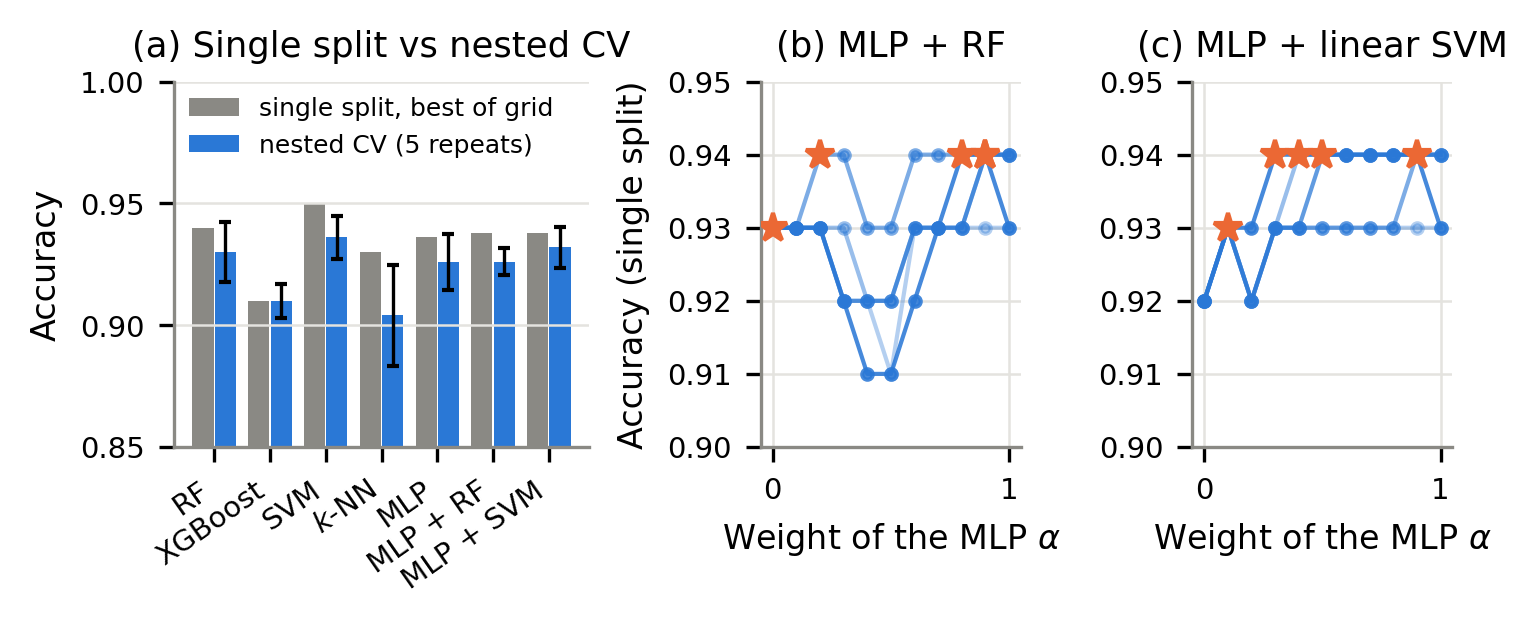
\includegraphics[width=\linewidth]{figs/protocol.png}
  \caption{(a) Best single-split accuracy and nested-CV accuracy (mean $\pm$ std over 5 repeats) of the same models and grids (21 volumetric features). (b, c) Accuracy of the soft vote (Eq.~\ref{eq:softvote}) on a single split as a function of $\alpha$, for five random seeds of the MLP ensemble (one curve each); stars mark the best $\alpha$ of each curve.}
  \label{fig:protocol-study}
\end{figure}

\subsection{Reconstruction of the LV cavity}
\label{sec:lv}
Filling the holes of the myocardium recovers the true cavity almost perfectly: 193 of the 200 training volumes are reconstructed voxel for voxel, and the mean Dice coefficient \citep{dice1945} is 0.997 (Table~\ref{tab:lv}). The 7 other volumes each miss one slice, the most basal one, where the myocardium is open (Figure~\ref{fig:lv}a, b). The volume error then reaches 29 mL and the ejection-fraction error 12.8 points, enough to move a patient across a diagnostic threshold. The convex-hull fallback recovers all 7 slices (minimum Dice 0.990, maximum ejection-fraction error 0.8 points). Without the area threshold, it also creates 20 spurious slices on apical caps; with a threshold of 25\% or 50\% of the myocardium area, it creates none. On the test set, the fallback never triggers: all test slices with myocardium are either closed rings or caps, so both methods give exactly the same test cavities.

% Generated by regenerate_figures.py from final/results/lv_reconstruction/tables/summary.csv
\begin{table}[!htb]
\centering
\small
\setlength{\tabcolsep}{4pt}
\begin{adjustbox}{max width=\linewidth}
\begin{tabular}{lrrrrrrrr}
\toprule
& \multicolumn{2}{c}{Dice} & Exact & Max $|\Delta V|$ & \multicolumn{2}{c}{Slices} & \multicolumn{2}{c}{$|\Delta$EF$|$ (points)}\\
\cmidrule(lr){2-3}\cmidrule(lr){6-7}\cmidrule(lr){8-9}
Method & mean & min & volumes & (mL) & missed & spurious & mean & max\\
\midrule
Filling (holes of the myocardium) & 0.9969 & 0.832 & 193 & 28.7 & 7 & 0 & 0.57 & 12.8\\
+ convex hull, no threshold & 0.9995 & 0.988 & 175 & 3.1 & 0 & 20 & 0.07 & 0.8\\
+ convex hull, area $\geq$ 25\% (ours) & 0.9998 & 0.990 & 193 & 3.1 & 0 & 0 & 0.03 & 0.8\\
+ convex hull, area $\geq$ 50\% & 0.9998 & 0.990 & 193 & 3.1 & 0 & 0 & 0.03 & 0.8\\
\bottomrule
\end{tabular}
\end{adjustbox}
\caption{Reconstruction of the LV cavity on the 200 training volumes (100 patients, ED and ES), compared with the
true LV. \emph{Exact}: volumes reconstructed voxel for voxel. EF errors are per patient.}
\label{tab:lv}
\end{table}


\begin{figure}[!htb]
  \centering
  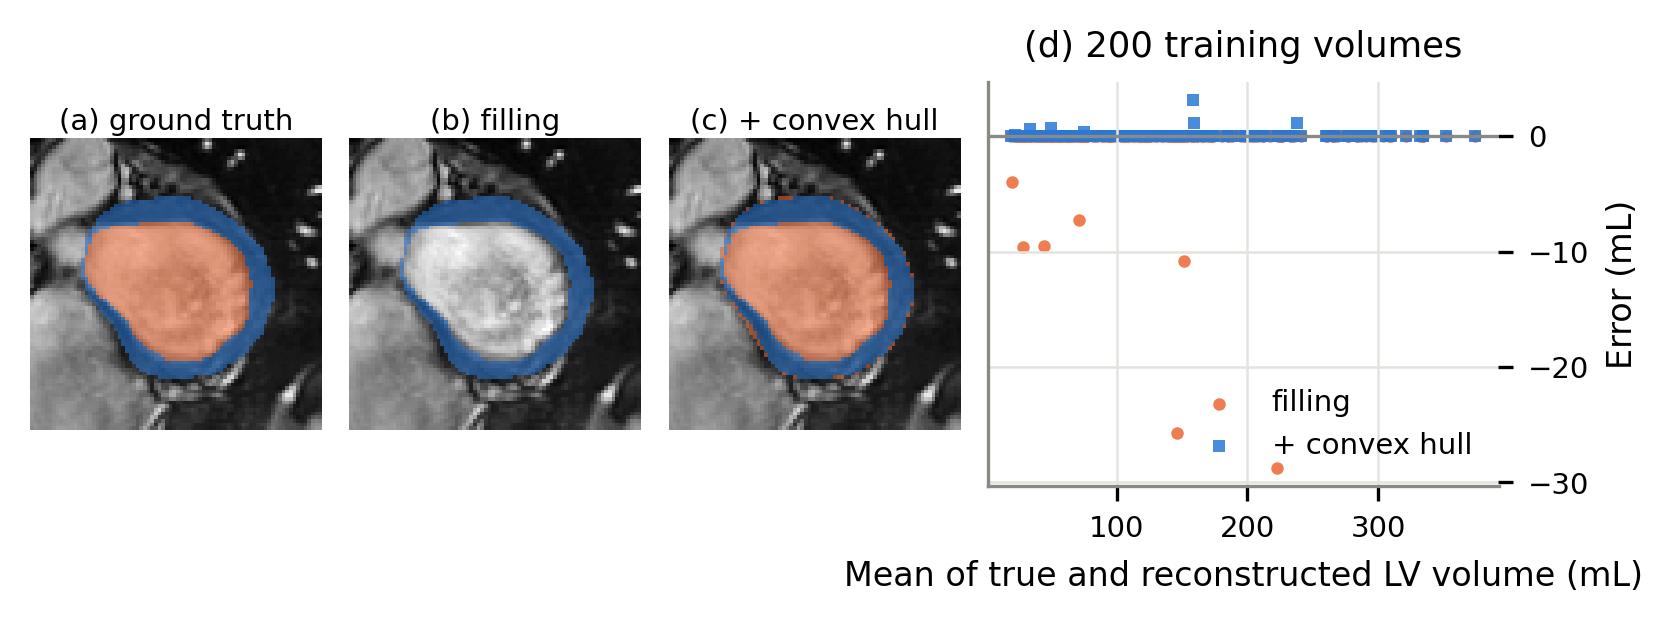
\includegraphics[width=\linewidth]{figs/lv_reconstruction.png}
  \caption{(a--c) Basal slice of training patient 011 at ED, whose myocardium does not close around the cavity: true cavity, filling (no cavity on this slice) and convex-hull fallback. (d) Error of the reconstructed LV volume against the mean of the true and reconstructed volumes \citep{blandaltman1986}, for the 200 training volumes.}
  \label{fig:lv}
\end{figure}

\subsection{Consistency of training and test features}
\label{sec:protocol}
A natural approach is to train the classifiers on features computed with the true LV, available for the training patients, and to apply them to test features computed with a reconstructed LV. To measure the effect of this mismatch, we train on one LV source and evaluate on another, for the same training patients (Table~\ref{tab:protocol}). The differences between protocols are at most 1.6 points and have no consistent sign: the linear SVM on 32 features scores 0.954, 0.956, 0.959 and 0.956 under the four protocols. Only 7 of the 100 training patients have features that differ at all between the true and reconstructed LV (Appendix~\ref{app:lv}); the largest changes, up to 98\% of the ejection fraction of one patient, occur with the filling without fallback. This mismatch is therefore harmless on this data. We nevertheless train and evaluate with \emph{fill+hull}, the same reconstruction as for the test patients.

% Generated by regenerate_figures.py from final/results/lv_protocol/tables/summary_mean.csv
\begin{table}[!htb]
\centering
\small
\setlength{\tabcolsep}{4pt}
\begin{adjustbox}{max width=\linewidth}
\begin{tabular}{lcccc}
\toprule
LV of training $\to$ evaluated patients & true $\to$ true & true $\to$ fill & fill $\to$ fill & fill+hull $\to$ fill+hull\\
\midrule
\multicolumn{5}{l}{\emph{Volumetric (21)}}\\
\quad Logistic regression & 0.897 $\pm$ 0.018 & 0.900 $\pm$ 0.014 & 0.900 $\pm$ 0.016 & 0.896 $\pm$ 0.016\\
\quad Linear SVM & 0.928 $\pm$ 0.014 & 0.928 $\pm$ 0.015 & 0.925 $\pm$ 0.014 & 0.925 $\pm$ 0.016\\
\quad Random forest & 0.922 $\pm$ 0.014 & 0.929 $\pm$ 0.015 & 0.932 $\pm$ 0.014 & 0.923 $\pm$ 0.016\\
\quad XGBoost & 0.918 $\pm$ 0.015 & 0.927 $\pm$ 0.013 & 0.928 $\pm$ 0.013 & 0.920 $\pm$ 0.013\\
\multicolumn{5}{l}{\emph{Volumetric + thickness (32)}}\\
\quad Logistic regression & 0.943 $\pm$ 0.014 & 0.937 $\pm$ 0.012 & 0.937 $\pm$ 0.012 & 0.953 $\pm$ 0.014\\
\quad Linear SVM & 0.954 $\pm$ 0.013 & 0.956 $\pm$ 0.013 & 0.959 $\pm$ 0.007 & 0.956 $\pm$ 0.014\\
\quad Random forest & 0.938 $\pm$ 0.012 & 0.944 $\pm$ 0.012 & 0.941 $\pm$ 0.014 & 0.938 $\pm$ 0.015\\
\quad XGBoost & 0.915 $\pm$ 0.020 & 0.922 $\pm$ 0.019 & 0.928 $\pm$ 0.020 & 0.916 $\pm$ 0.021\\
\bottomrule
\end{tabular}
\end{adjustbox}
\caption{Effect of the LV used to compute the features (nested CV, 10 repeats). \emph{true}: ground-truth LV
(training set only); \emph{fill}: filling; \emph{fill+hull}: filling with the convex-hull fallback.
``true $\to$ fill'' is the situation of a model trained with the true LV and applied to the test set.}
\label{tab:protocol}
\end{table}


\subsection{Comparison of features and classifiers}
\label{sec:bench}
Table~\ref{tab:benchmark} and Figure~\ref{fig:bench} compare 10 classifiers on the three feature sets. On the 21 volumetric features, accuracies range from 0.895 ($k$-NN) to 0.931 (extra trees), and the ensembles do not beat their components. Adding the 11 thickness features improves most models: logistic regression by 5.7 points, the MLP ensemble by 3.7, the linear SVM by 3.1 and MLP + linear SVM by 3.9. The trees gain little (random forest +1.5, extra trees +0.6) and XGBoost does not gain at all. The best configuration is MLP + linear SVM on the 32 features, with $0.966 \pm 0.011$. Its paired advantage over the MLP ensemble alone is $0.009 \pm 0.008$, and over the linear SVM alone $0.010 \pm 0.009$, i.e.\ one patient on average. The compact set (12 features) reaches 0.955 with the same ensemble. It gives the best HCM recall (1.00 for logistic regression and the RBF SVM), but loses MINF patients (recall 0.89 to 0.91 for the linear models, SVMs and MLP ensembles, against 0.95 to 0.96 with 32 features; Appendix~\ref{app:bench}).

% Generated by regenerate_figures.py from final/results/benchmark/tables/summary_mean.csv
\begin{table}[!htb]
\centering
\small
\setlength{\tabcolsep}{5pt}
\begin{tabular}{lccc}
\toprule
Model & Volumetric (21) & Volumetric + thickness (32) & Compact (12)\\
\midrule
Logistic regression & 0.896 $\pm$ 0.016 & 0.953 $\pm$ 0.014 & 0.942 $\pm$ 0.015\\
Linear SVM & 0.925 $\pm$ 0.016 & 0.956 $\pm$ 0.014 & 0.927 $\pm$ 0.009\\
RBF SVM & 0.923 $\pm$ 0.022 & 0.945 $\pm$ 0.012 & 0.944 $\pm$ 0.019\\
$k$-NN & 0.895 $\pm$ 0.010 & 0.902 $\pm$ 0.023 & 0.932 $\pm$ 0.012\\
\midrule
Random forest & 0.923 $\pm$ 0.016 & 0.938 $\pm$ 0.015 & 0.925 $\pm$ 0.019\\
Extra trees & \textbf{0.931} $\pm$ 0.010 & 0.937 $\pm$ 0.012 & 0.940 $\pm$ 0.009\\
XGBoost & 0.920 $\pm$ 0.013 & 0.916 $\pm$ 0.021 & 0.915 $\pm$ 0.022\\
\midrule
MLP ensemble & 0.920 $\pm$ 0.012 & 0.957 $\pm$ 0.008 & 0.953 $\pm$ 0.014\\
MLP + RF & 0.925 $\pm$ 0.012 & 0.954 $\pm$ 0.010 & 0.952 $\pm$ 0.019\\
MLP + linear SVM & 0.927 $\pm$ 0.012 & \textbf{0.966} $\pm$ 0.011 & \textbf{0.955} $\pm$ 0.008\\
\bottomrule
\end{tabular}
\caption{Nested-CV accuracy (mean $\pm$ std over 10 repeats of stratified 5-fold CV) with the LV reconstructed in
training and evaluated patients, as for the test set. Hyper-parameters and the ensemble weight $\alpha$ are
selected by an inner 5-fold CV. Best value of each column in bold. Classes are balanced, so the balanced accuracy
equals the accuracy.}
\label{tab:benchmark}
\end{table}


\begin{figure}[!htb]
  \centering
  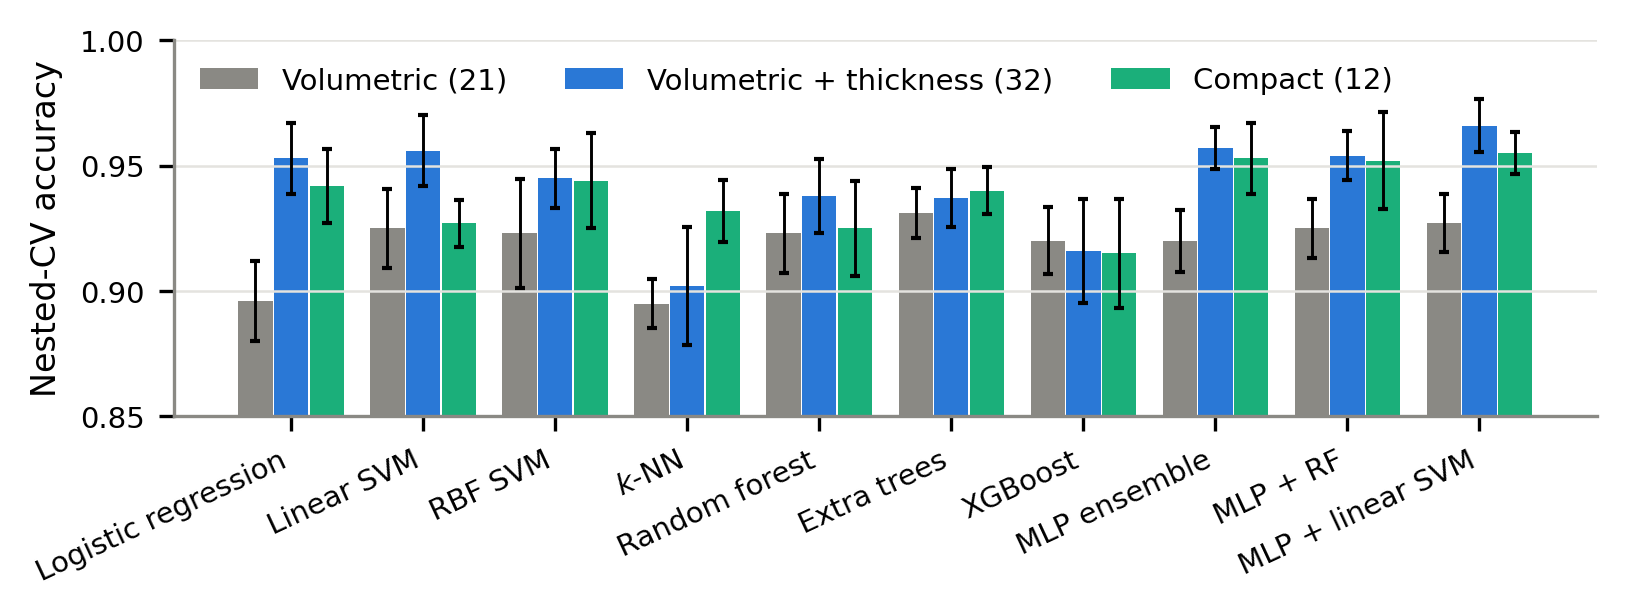
\includegraphics[width=\linewidth]{figs/benchmark.png}
  \caption{Nested-CV accuracy of each classifier on the three feature sets (mean $\pm$ std over 10 repeats).}
  \label{fig:bench}
\end{figure}

Figure~\ref{fig:features} shows why the thickness features help. The LV ejection fraction and indexed volume separate the groups with a dilated, poorly contracting LV (MINF and DCM) from the others, and the RV ejection fraction isolates ARV and part of DCM. The myocardial mass separates HCM and DCM from the others, but not from each other. The thickest slice at ED isolates HCM. The variability of the wall thickness within a slice at ES is high for HCM and MINF and low for DCM: an infarct thins one segment of the wall and leaves the others thick, while a dilated cardiomyopathy thins the whole wall evenly. This feature thus separates MINF from DCM, the pair that the volumes confuse most.

\begin{figure}[!htb]
  \centering
  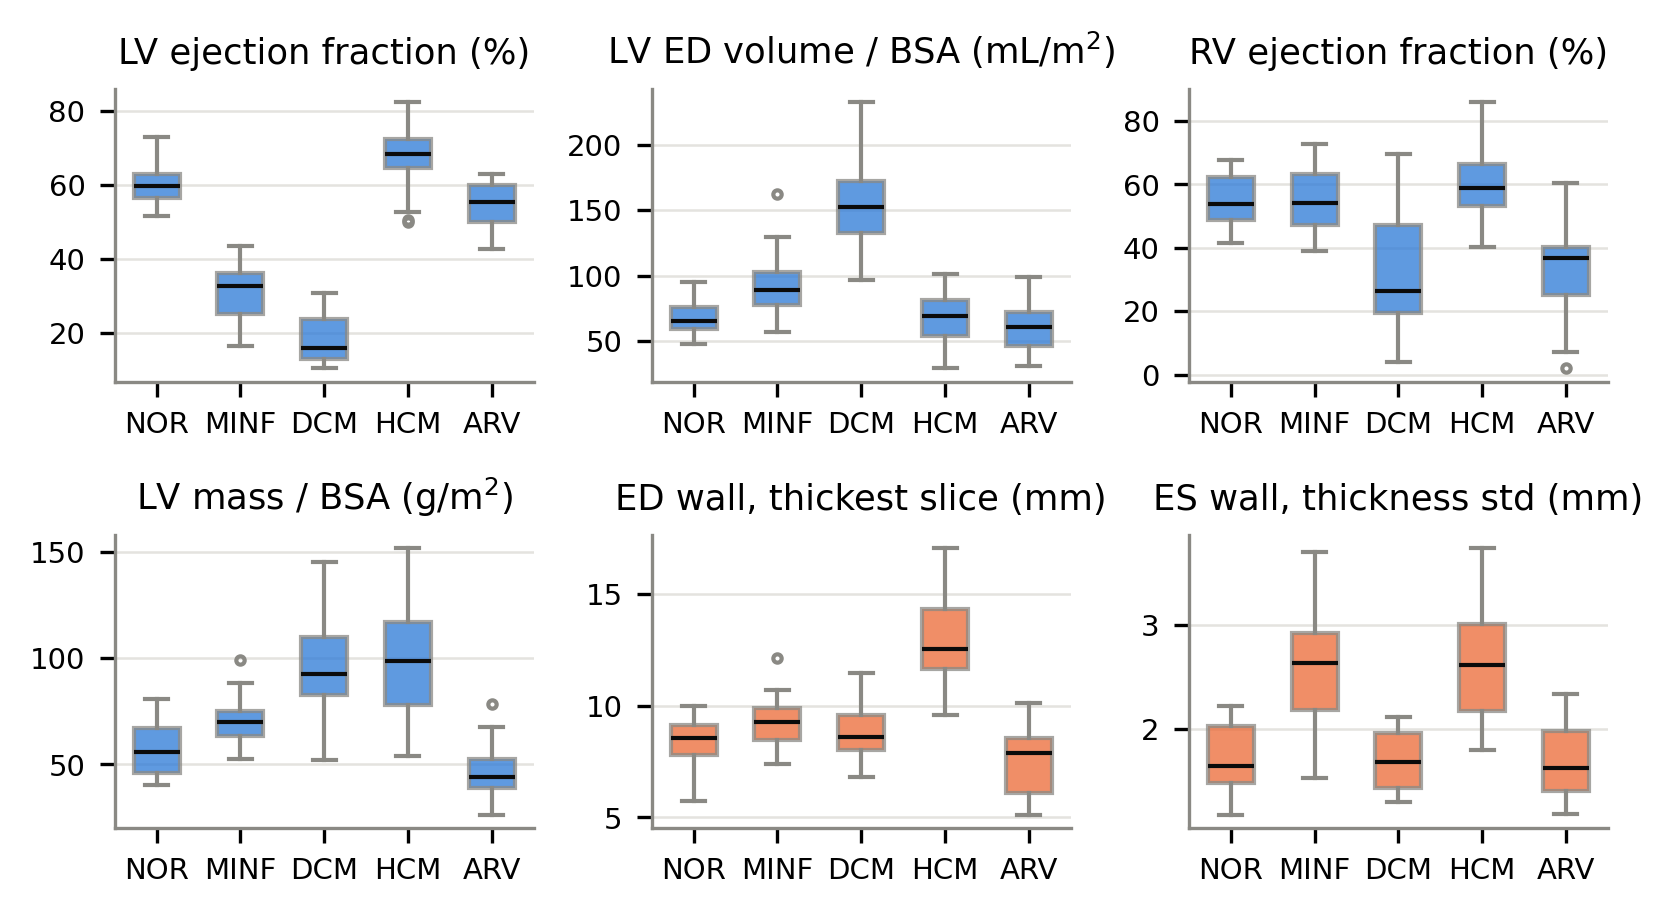
\includegraphics[width=\linewidth]{figs/features_by_class.png}
  \caption{Distribution of six features per group (100 training patients, reconstructed LV). Blue: volumetric features; orange: thickness features. Boxes: quartiles; whiskers: 1.5 times the interquartile range.}
  \label{fig:features}
\end{figure}

\subsection{Final model}
\label{sec:final}
The final model is the soft vote of the MLP ensemble and a linear SVM ($C=1$) on the 32 features, with the LV reconstructed by \emph{fill+hull}. The inner cross-validation selects $\alpha=0.5$ in 33 of the 50 outer folds and on the whole training set. Its nested-CV accuracy is $0.966 \pm 0.011$ (0.94 to 0.98 over the repeats), with recalls between 0.945 (DCM) and 0.985 (NOR) (Figure~\ref{fig:final}a; Appendix~\ref{app:final}).

\paragraph{Errors}
Over the 10 repeats, 9 patients are misclassified at least once, and only 3 more than twice. MINF patient 050 is always predicted DCM: its LV ejection fraction is 16\% and its indexed ED volume 163 mL/m$^2$, the values of a typical DCM. DCM patient 002 is predicted MINF in 9 repeats out of 10, with an unusually uneven wall for a DCM. HCM patient 022 is predicted NOR in 4 repeats and MINF in 1; its ejection fraction (65\%) and wall thickness lie between those of the NOR and HCM groups. The MINF / DCM confusion is clinically expected: an extensive infarct can dilate the LV until it resembles a dilated cardiomyopathy, and conversely, and the two are told apart by the localization of the lesion (late gadolinium enhancement), which segmentations do not show.

\paragraph{Feature importance}
Permuting the within-slice variability of the ES wall thickness costs 5 points of held-out accuracy, twice as much as any other feature (Figure~\ref{fig:final}b). The LV and RV ejection fractions, the stroke volume and the RV volume at ES follow. Many features are strongly correlated (volumes and their indexed versions, the two mass / volume ratios), so the importance of each is shared with its correlates \citep{strobl2007}, and the standard deviations are large.

\begin{figure}[!htb]
  \centering
  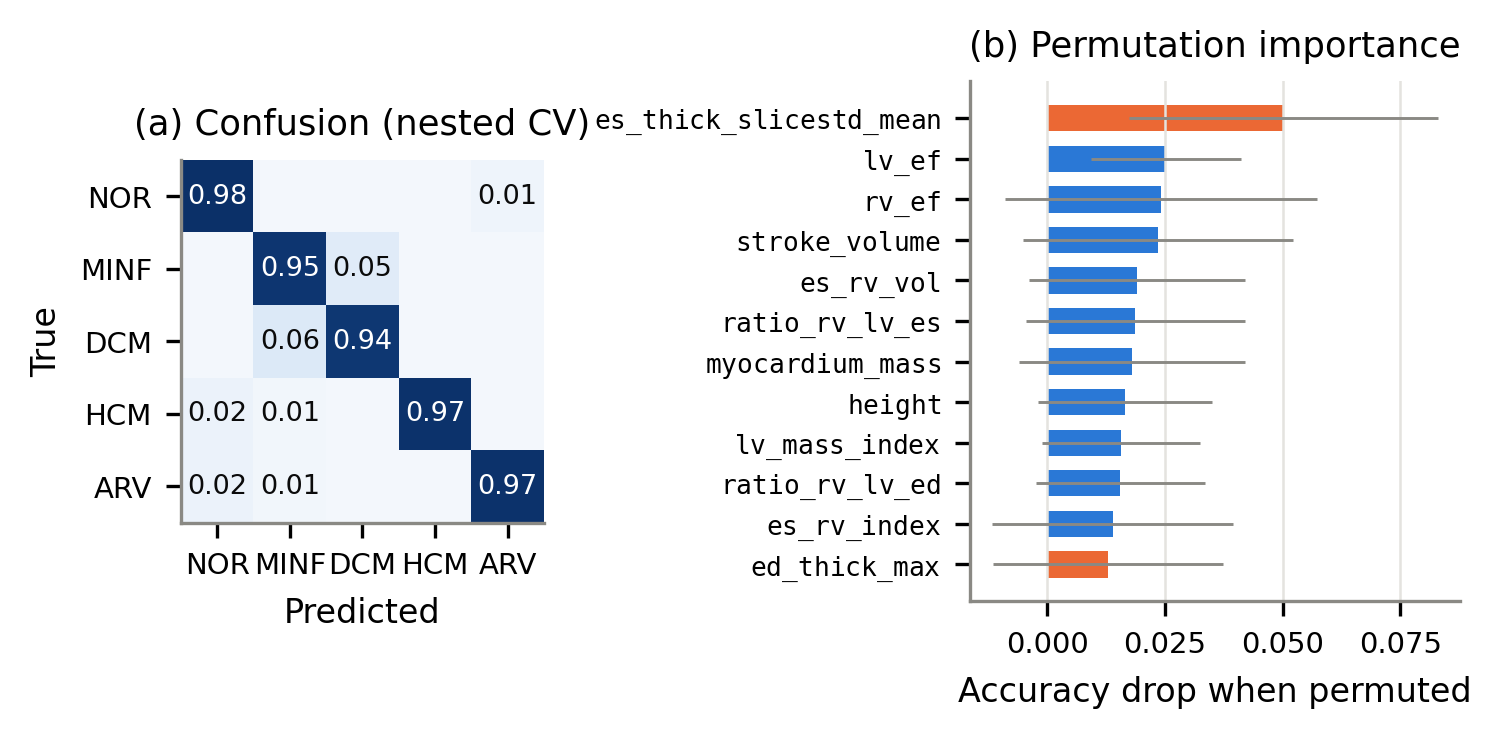
\includegraphics[width=\linewidth]{figs/final_model.png}
  \caption{Final model. (a) Confusion matrix pooled over the 10 repeats of the nested cross-validation (rows sum to 1). (b) Permutation importance of the 12 most important features on held-out folds (mean $\pm$ std over 15 folds); orange: thickness features.}
  \label{fig:final}
\end{figure}

\paragraph{Test predictions}
Fitted on the 100 training patients, the model predicts 12 NOR, 8 MINF, 11 DCM, 9 HCM and 10 ARV patients among the 50 test patients, close to the 10 per group of the ACDC test set. The mean probability of the predicted class is 0.81, and 6 patients have a probability below 0.6. These predictions cannot be scored here: the test labels are hidden behind the course leaderboard (Appendix~\ref{app:final}).
